\documentclass{beamer}
\usepackage[latin1]{inputenc}
\usepackage{amssymb}
\usepackage{subfigure}
\usetheme{Warsaw}
\title[The Dependence of Planning Horizon on Model Accuracy]{The Dependence of Effective Planning Horizon on Model Accuracy}
\author[]{David Abel  \and Enrique Areyan \\ Kavosh Asadi  \and David Hershkowitz}
\date{December 15, 2015}
\begin{document}

% Title Slide
\begin{frame}
\titlepage
\end{frame}

% Dave/Ellis vote we don't include an outline since it's only 5 minutes.
%% Slide: What is the point?
\begin{frame}{Outline}
\begin{enumerate}
	\item What is the point?
	\item Background
	\item RandomMDP Story
	\item RandomMDP Results
	\item UCT Story
	\item Rock Sample Domain
	\item UCT Results
	\item UCT Reproducibility Discussion
\end{enumerate}
\end{frame}

% Slide: What is the point?
\begin{frame}{What is the Point?}
\centering
Planning Depth should be determined proportionally to model accuracy
%An Innacurate
%With limited data 
%With an inaccurate model use a low planning Depth
\end{frame}


% Slide: RandomMDP Story
\begin{frame}{RandomMDP Story}
The evaluation is performed on a MDP designed by the authors, called RandomMDP, specified as:
\begin{enumerate}
\item 10 states, 2 actions
\item choose next state uniformly random from 5 possible states
\item rewards $~$ uniform(0,1), sample rewards have additive Gaussian noise
\end{enumerate}
Evaluation approach:


\end{frame}

% Slide: RandomMDP Results
\begin{frame}{RandomMDP Results}
\begin{tabular}{cc}
our results & their results \\
	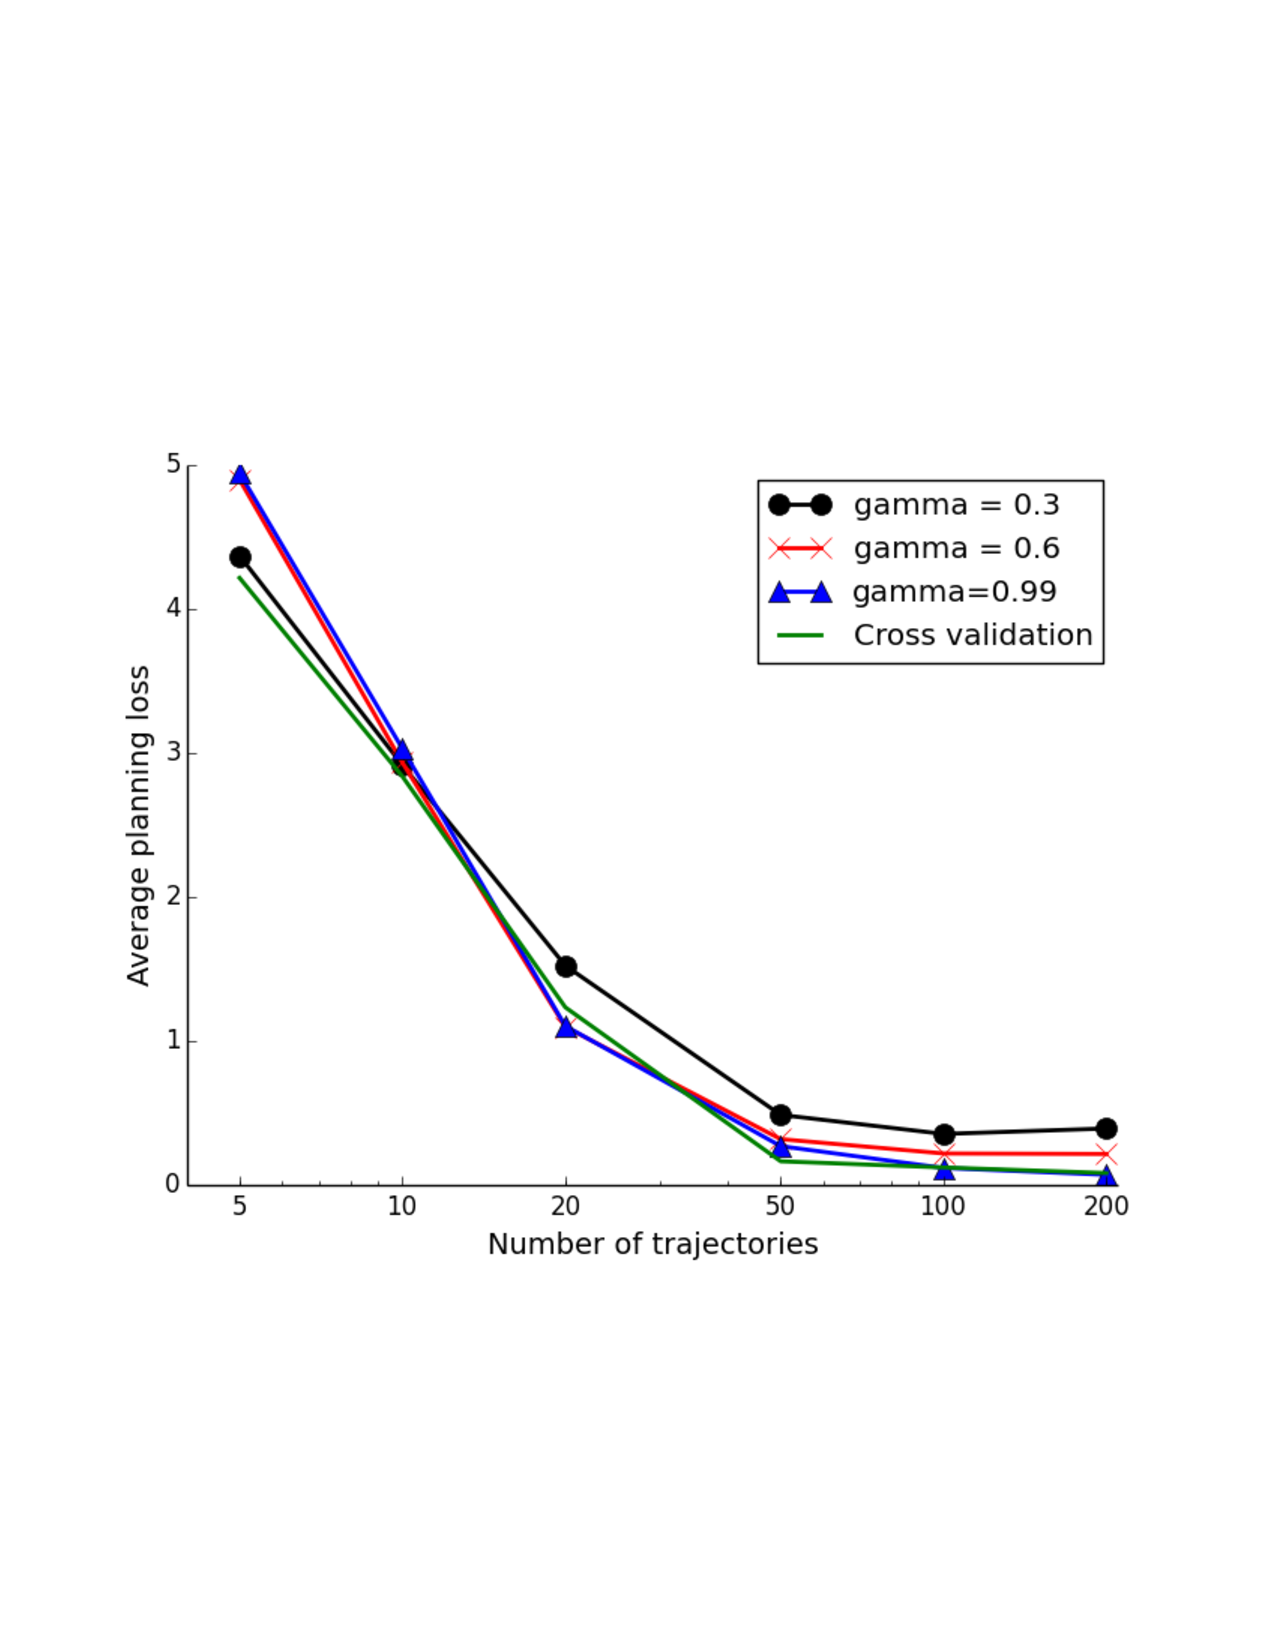
\includegraphics[page=1,height=.55\textheight,width=.5\textwidth]{../results/figure_2.pdf} &
	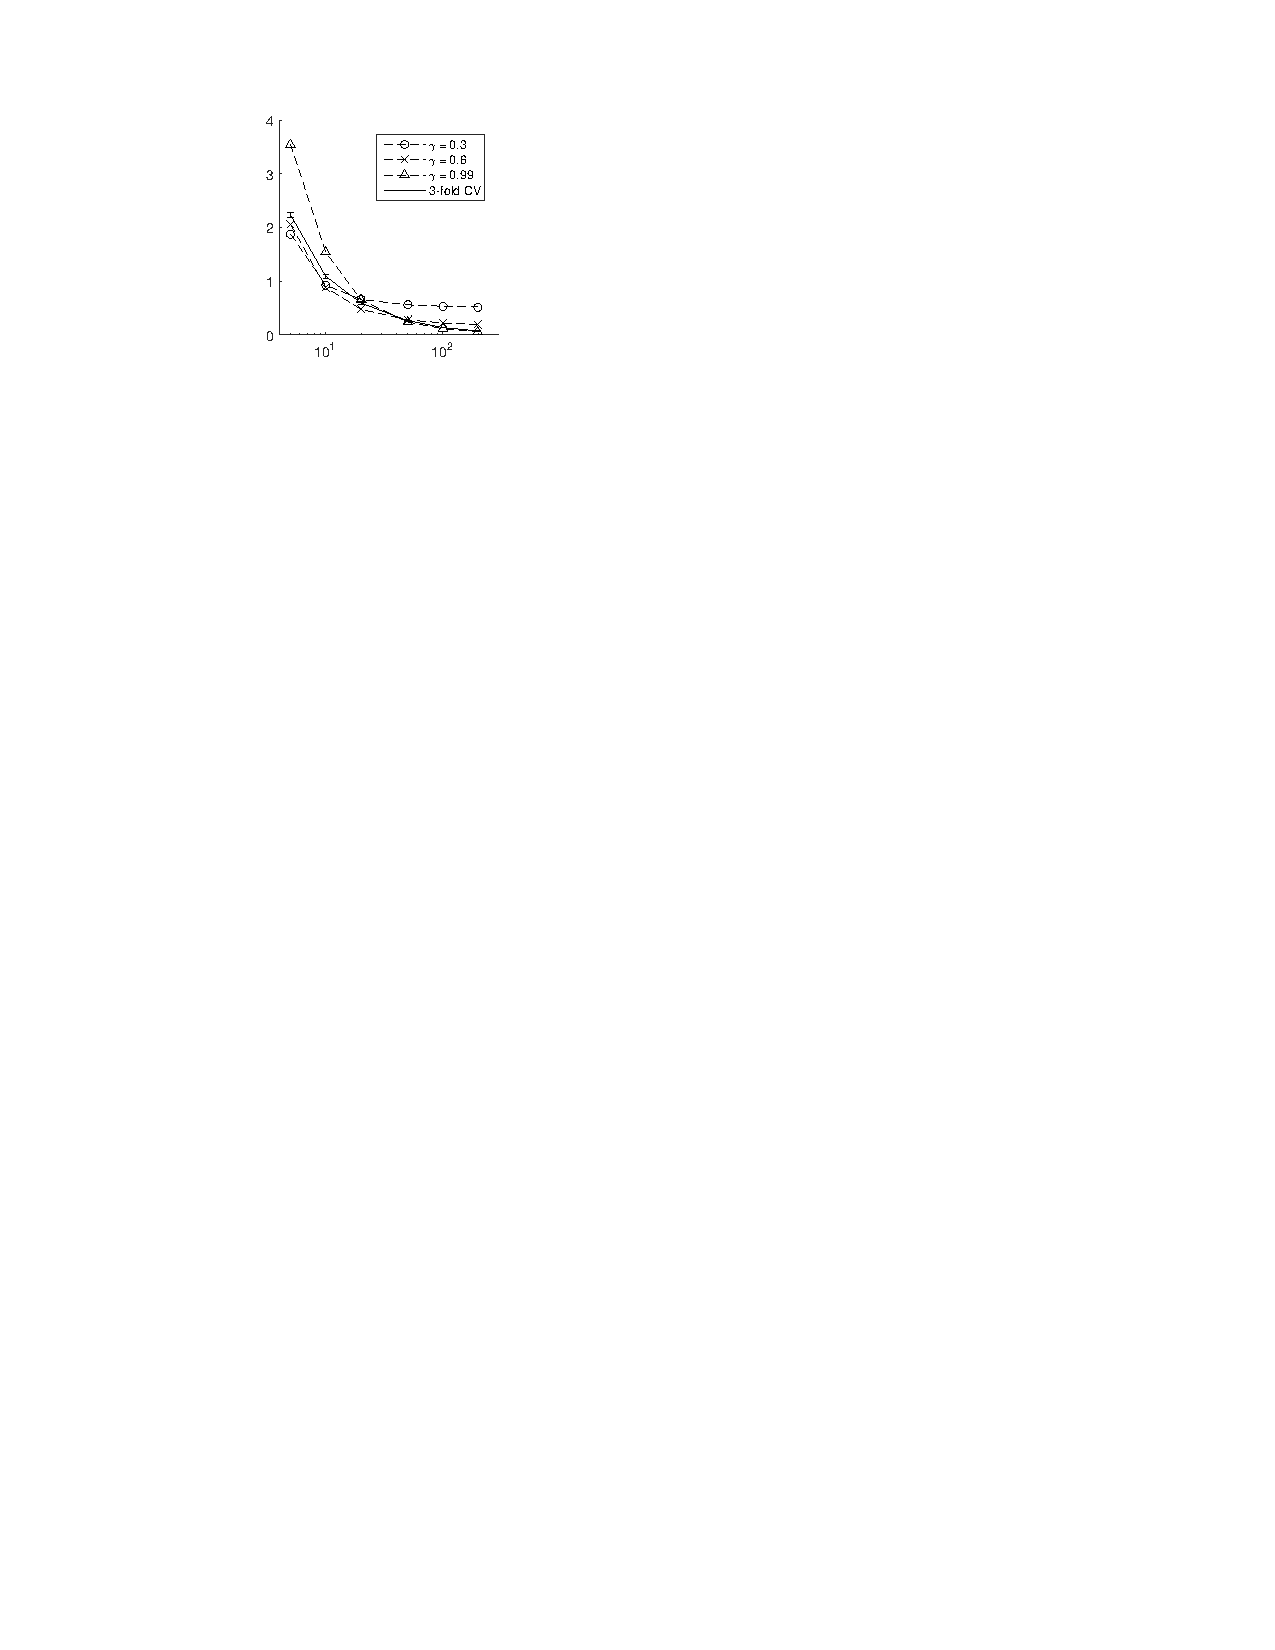
\includegraphics[page=1,width=.41\textwidth]{../results/originalCV.pdf}
\end{tabular}
\end{frame}



% Slide: UCT Story
\begin{frame}{UCT Story}
UCT: 
\begin{itemize}
\item UCB
\item Monte Carlo Planning
% \item Planning Depth and $\gamma$
\end{itemize}

Experiments:
\begin{itemize}
\item Rock Sample Domain
\item Comparing UCT performance with different planning depths.
\end{itemize}
\end{frame}

% Slide: UCT Story
\begin{frame}{Rock Sample Domain}

\begin{figure}
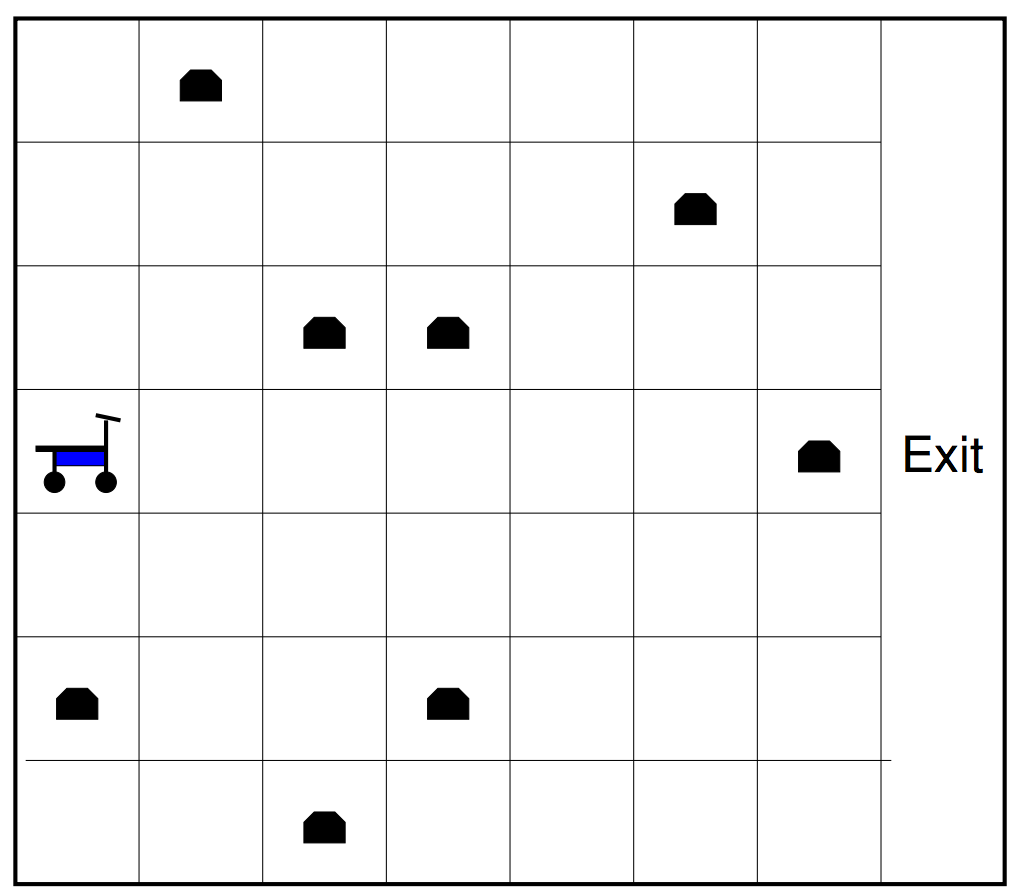
\includegraphics[page=1,height=.55\textheight,width=.5\textwidth]{rock_sample_domain.png}
\end{figure}


\end{frame}

% UCT Results
\begin{frame}{UCT Results}
\begin{figure}[h]
\centering
\subfigure[Our results]{
\label{fig: UCTOurResults}
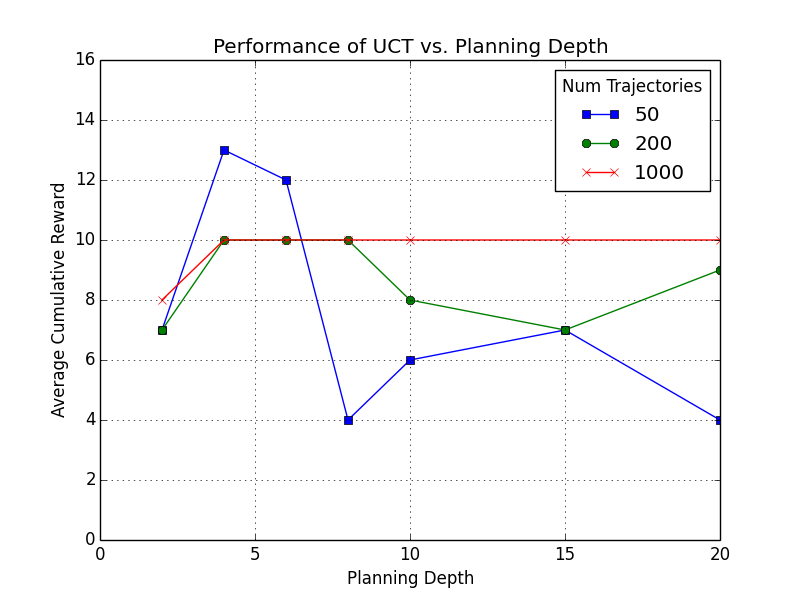
\includegraphics[page=1,width=.48\textwidth]{../results/rock_sample_results.png}}
\hspace{1mm}
\subfigure[Their results]{
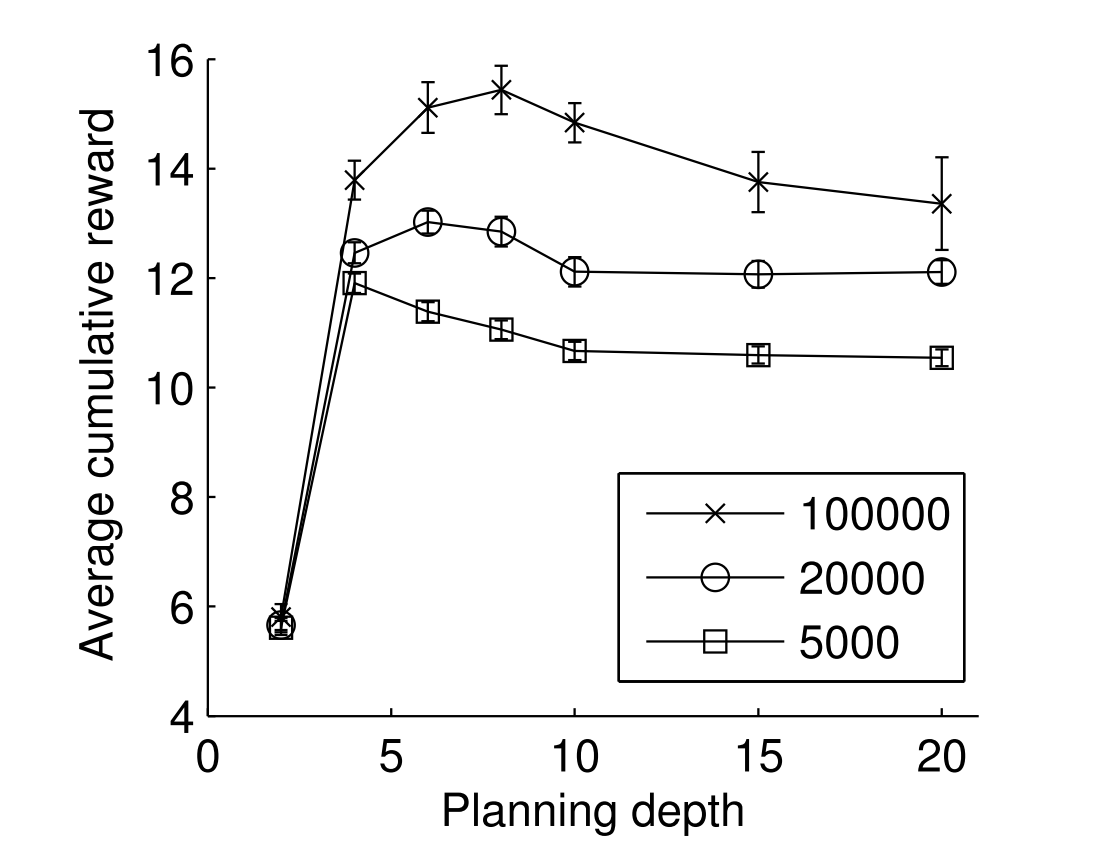
\includegraphics[page=1,width=.46\textwidth]{../results/figure_6.png}}
\end{figure}
\end{frame}

% Slide: Reproducbility Discussion
\begin{frame}{UCT Reproducibility Discussion}
\begin{itemize}
\item Ambiguities of UCT
\item Ambiguities of Rock Sample
\item Computational Limitations
\end{itemize}
\end{frame}












\end{document}
